\chapter{Сэмплирование}
\label{ch:chap2}

\definecolor{codegreen}{rgb}{0,0.6,0}
\definecolor{codegray}{rgb}{0.5,0.5,0.5}
\definecolor{codepurple}{rgb}{0.58,0,0.82}
\definecolor{backcolour}{rgb}{0.95,0.95,0.92}

\lstdefinestyle{mystyle}{
    backgroundcolor=\color{backcolour},   
    commentstyle=\color{codegreen},
    keywordstyle=\color{magenta},
    numberstyle=\tiny\color{codegray},
    stringstyle=\color{codepurple},
    basicstyle=\ttfamily\footnotesize,
    breakatwhitespace=false,         
    breaklines=true,                 
    captionpos=b,                    
    keepspaces=true,                 
    numbers=left,                    
    numbersep=5pt,                  
    showspaces=false,                
    showstringspaces=false,
    showtabs=false,                  
    tabsize=2
}
\lstset{style=mystyle}

В этом задании будем исследовать теорему Найквиста-Шеннона-Котельникова. Для этого нам также пригодится интерполяционный полином:
$$f(t) = \sum_{n=-\infty}^{+\infty}f(t_n)\cdot sinc(2B(t-t_n))$$ , где $t_n = \frac{n}{2B}$, по сути мы ставим шаг в $1/2B$


\section{Сэмплирование синусов}

Рассматриваем функцию с параметрами $a_1, a_2, \omega_1, \omega_2, \phi_1, \phi_2$:
$$y(t) = a_1 sin(\omega_1 t + \phi_1) + a_2 sin(\omega_2 t+\phi_2)$$

Теперь зададим два вектора - времени $t$ и значений $y$. Вектор времени задаём с достаточно частым шагом, чтобы можно было имитировать непрерывную функцию.
После задаём сэмплированный вариант, для этого нам нужно будет указать подшаг, с которым мы будем отбирать точки. В данном случае для сэмпла мы брали: 18000 точек $\rightarrow$ 720 точек.

Для того, чтобы не вслепую определять $B$, посмотрим на его Фурье образ:

\begin{figure}[ht]
    \centering
    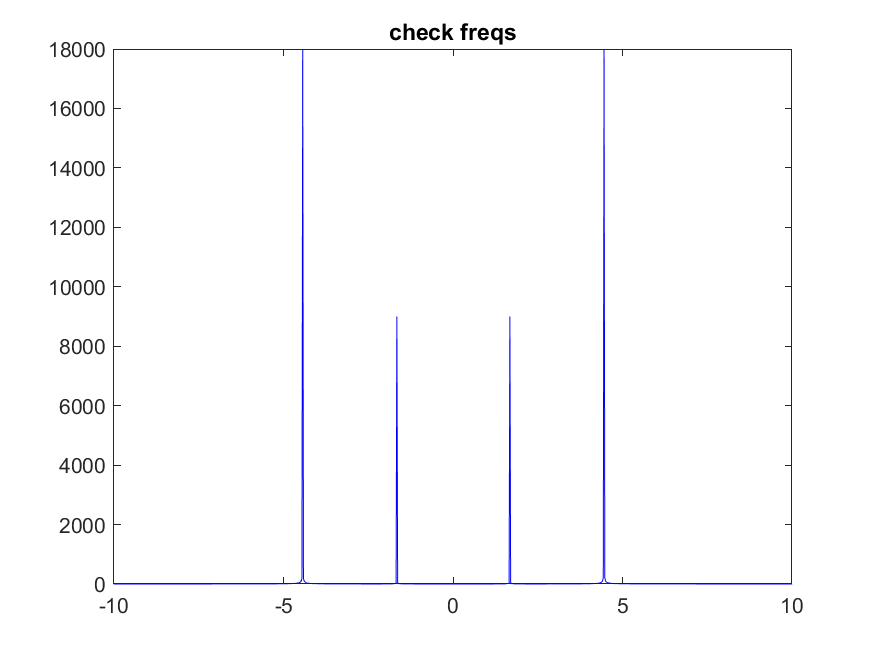
\includegraphics[width=0.7\textwidth]{2_check_freqs1.png}
	\caption{Смотрим Фурье}
\end{figure}

\begin{figure}[!ht]
	\centering
\hspace*{\fill}%
	\begin{subfigure}[b]{0.49\textwidth}
        \centering
		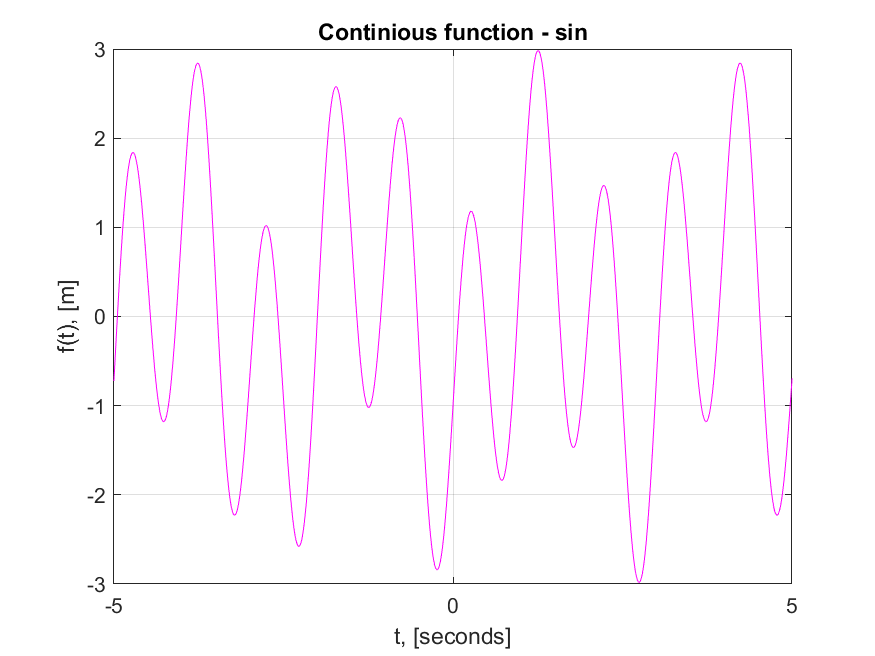
\includegraphics[width=1\textwidth]{2_1.png}
	\end{subfigure}
\hfill
	\begin{subfigure}[b]{0.49\textwidth}
        \centering
		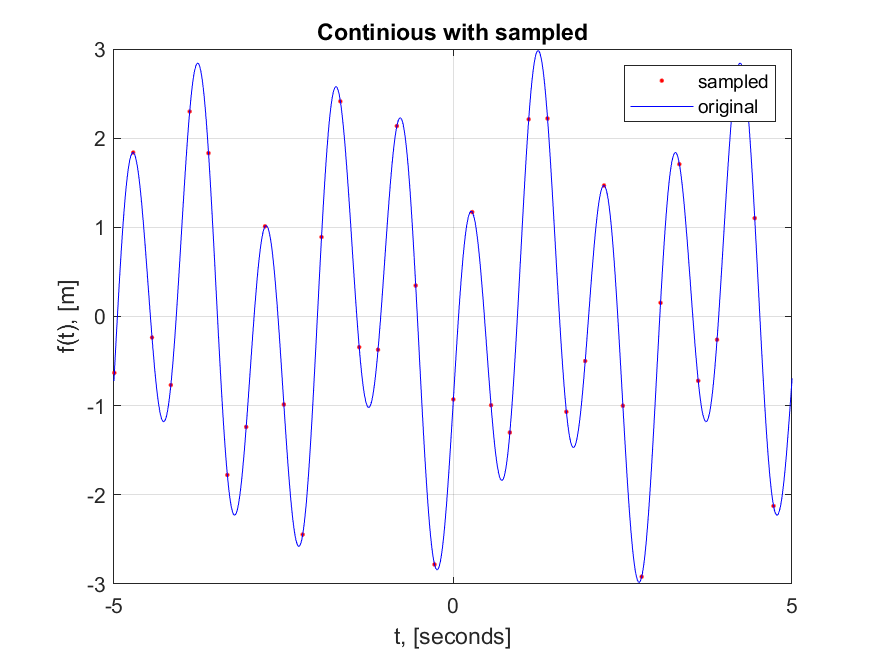
\includegraphics[width=1\textwidth]{2_2.png}
	\end{subfigure}
    \caption{Функция и её сэмплированный вариант}
\end{figure}
К этому сэмплу мы как раз будем применять интерполяционную формулу с разным шагом дискретизации:
\newpage
\begin{figure}[ht]
    \centering
    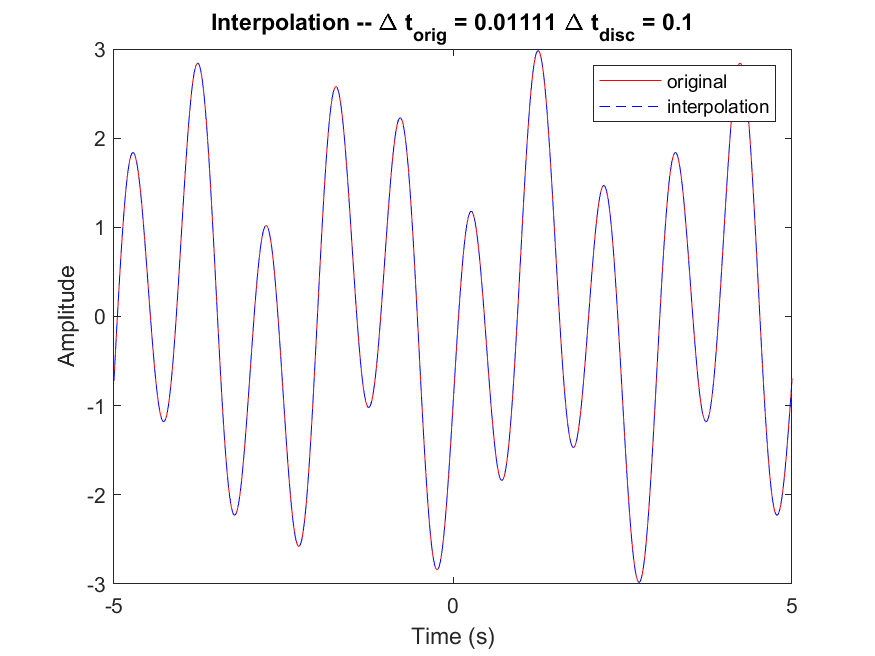
\includegraphics[width=0.7\textwidth]{2_3.png}
	\caption{Испытание 1 - B = 5}
\end{figure}


\begin{figure}[ht]
    \centering
    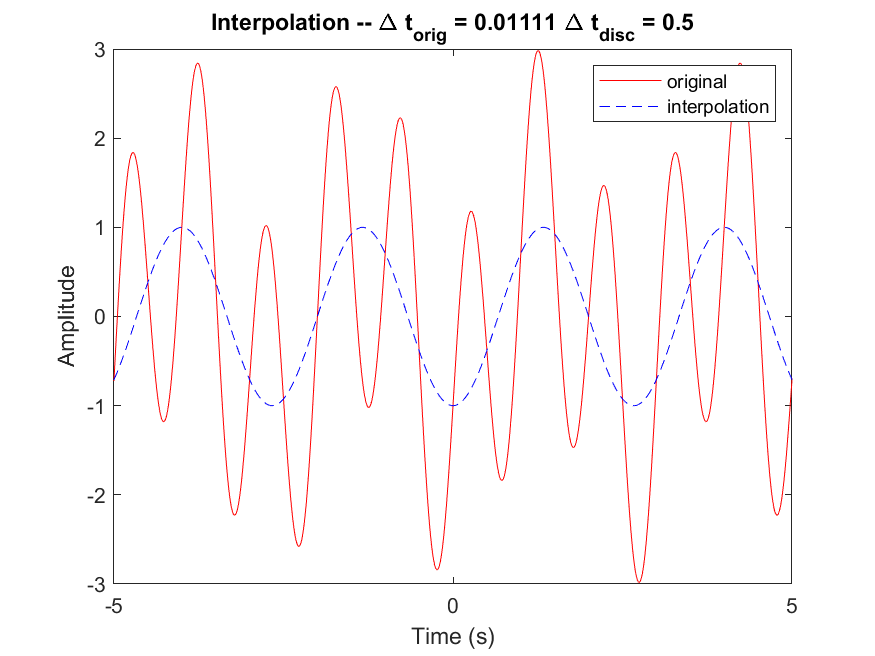
\includegraphics[width=0.7\textwidth]{2_4.png}
	\caption{Испытание 2 - B = 1}
\end{figure}

\begin{figure}[ht]
    \centering
    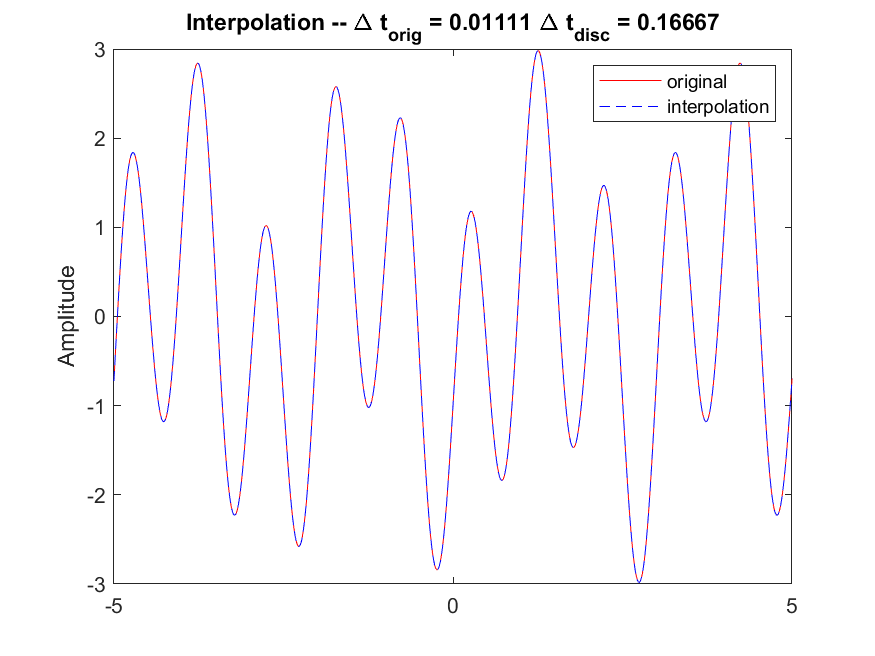
\includegraphics[width=0.7\textwidth]{2_5.png}
	\caption{Испытание 3 - B = 3}
\end{figure}

\begin{figure}[ht]
    \centering
    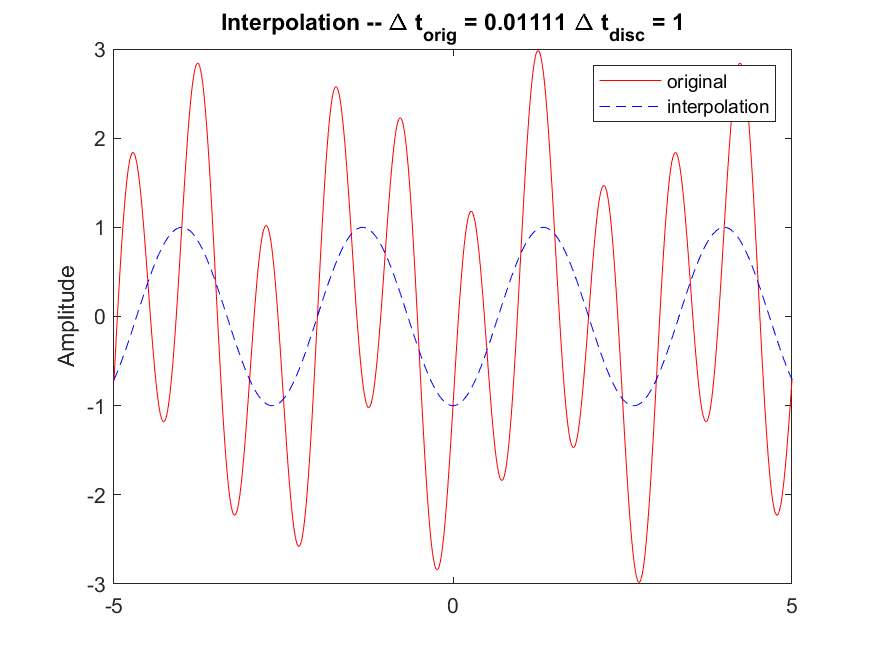
\includegraphics[width=0.7\textwidth]{2_6.png}
	\caption{Испытание 4 - B = 0.5}
\end{figure}
\newpage

Все испытания проводились с целью проверить с обоих сторон неравенство из теоремы: $\Delta t < \frac{1}{2B}$, где $\Delta t$ -  дискретный шаг времени, 
а $[-B; B]$ - конечный отрезок, в котором лежим весь Фурье образ. В моём случае $B\approx 5$, но я брал и больше и меньше, сравнивал что будет с исходной функцией. Когда мы берём больше - то очевидно, что функция восстанавливается очень хорошо, но не всё так просто, когда мы уменьшаем $B$ - там возникают аномалии, и функция может хорошо восстановиться,
а может - нет, катавасия какая-то... Поэтому лучше брать $B$ вперёд с запасом.

В итоге мы смогли подвердить, что выполняя неравенство из теоремы Найквиста-Шеннона-Котельникова мы можем восстановить исходную функцию по конечному, дискретному набору её значений (с маленьким допущением - её Фурье-образ конечен).

\section{Сэмплирование sinus cardinalis} % 18-->28 images

Рассматриваем функцию с параметром $b$, будьте осторожны - при $b>5$ функция очень быстро улетает в бесконечность:
$$y(t) = sinc(bt)$$

Посмотрим на функцию и её сэмплированный вариант (8000 точек $\rightarrow$ 6000 точек)

\begin{figure}[!ht]
	\centering
\hspace*{\fill}%
	\begin{subfigure}[b]{0.49\textwidth}
        \centering
		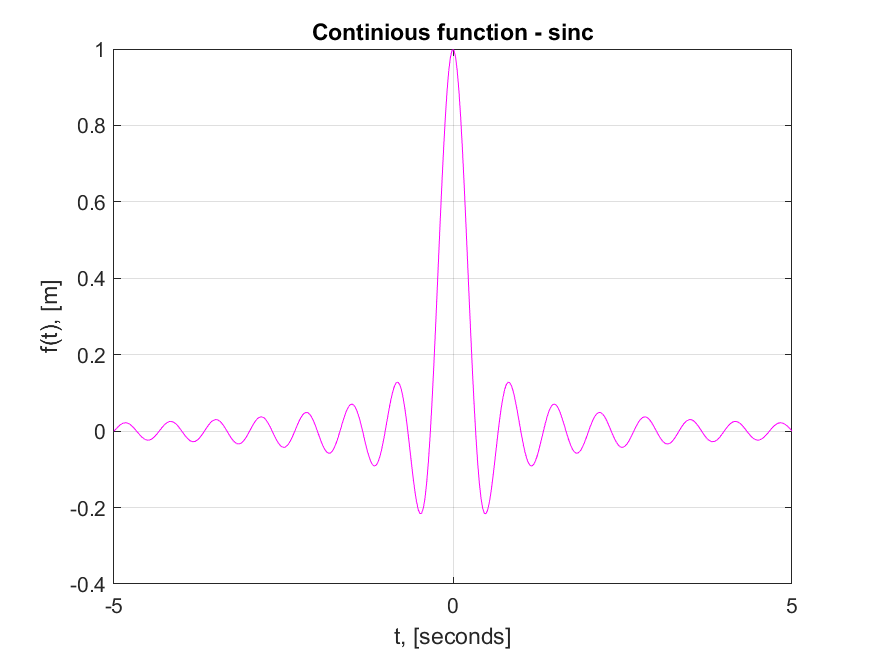
\includegraphics[width=1\textwidth]{2_18.png}
	\end{subfigure}
\hfill
	\begin{subfigure}[b]{0.49\textwidth}
        \centering
		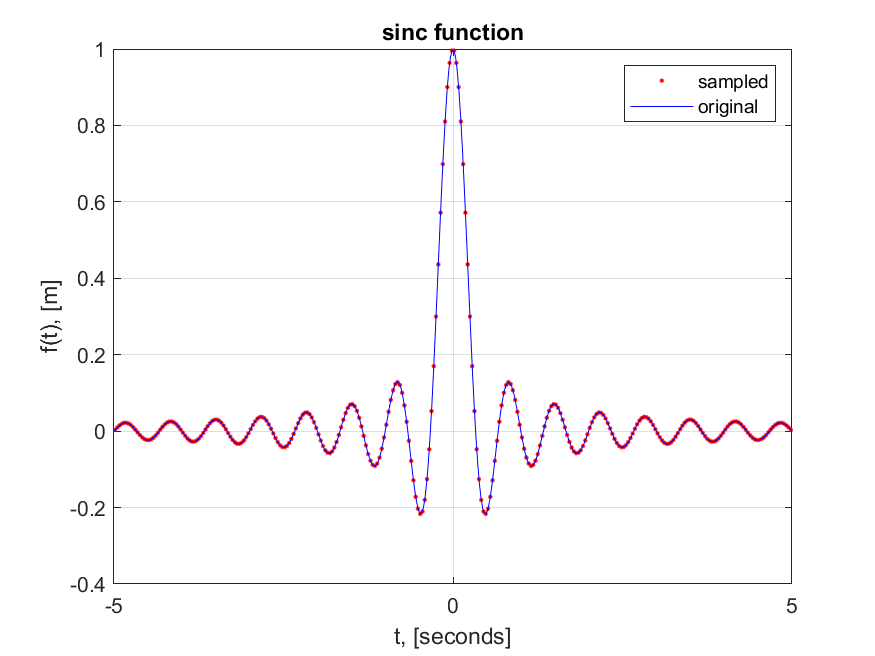
\includegraphics[width=1\textwidth]{2_19.png}
	\end{subfigure}
    \caption{Функция и её сэмплированный вариант}
\end{figure}

Теперь сравниваем как будут выглядеть образы оригинала и восстановленные, и то же самое с кардинальным синусом(оригинал и интерполированный), посмотрим как будет влиять шаг сэмпла на конечное восстановление функции

\begin{figure}[!ht]
	\centering
\hspace*{\fill}%
	\begin{subfigure}[b]{0.49\textwidth}
        \centering
		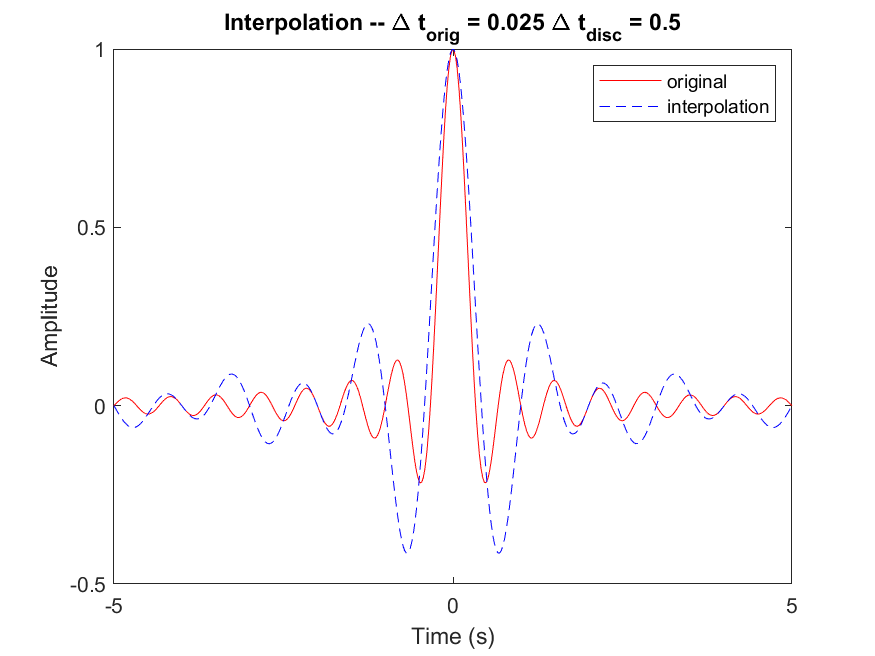
\includegraphics[width=1\textwidth]{2_21.png}
	\end{subfigure}
\hfill
	\begin{subfigure}[b]{0.49\textwidth}
        \centering
		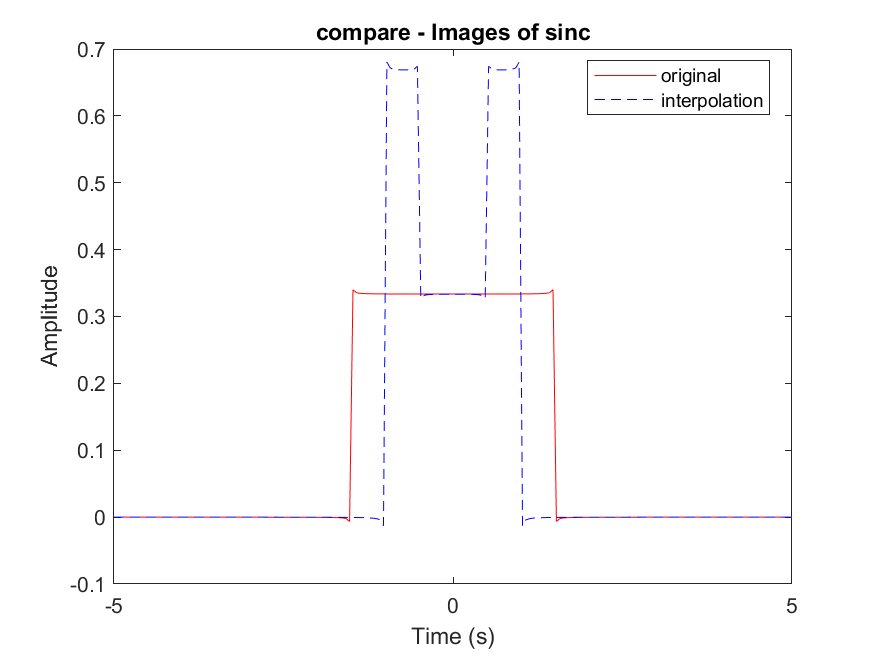
\includegraphics[width=1\textwidth]{2_22.png}
	\end{subfigure}
    \caption{ Испытание - 1 - B = 1}
\end{figure}
\newpage
Для того, чтобы подбирать $B$ было удобнее - давайте посмотрим на Образ Фурье - здесь я его специально приблизил, но так то он периодический.
\begin{figure}[ht]
    \centering
    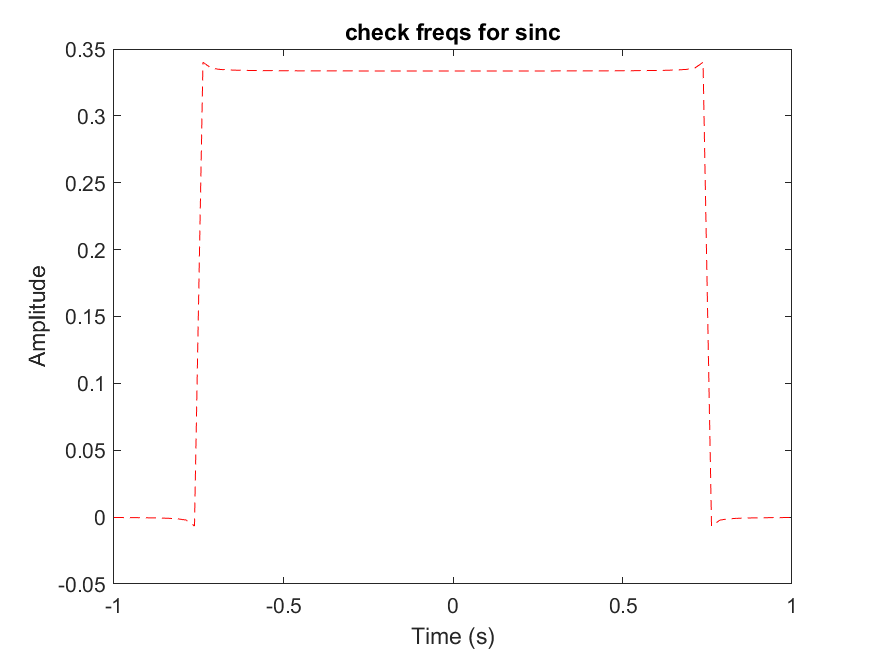
\includegraphics[width=0.6\textwidth]{2_20.png}
	\caption{Смотрим на образ}
\end{figure}

\begin{figure}[!ht]
	\centering
\hspace*{\fill}%
	\begin{subfigure}[b]{0.49\textwidth}
        \centering
		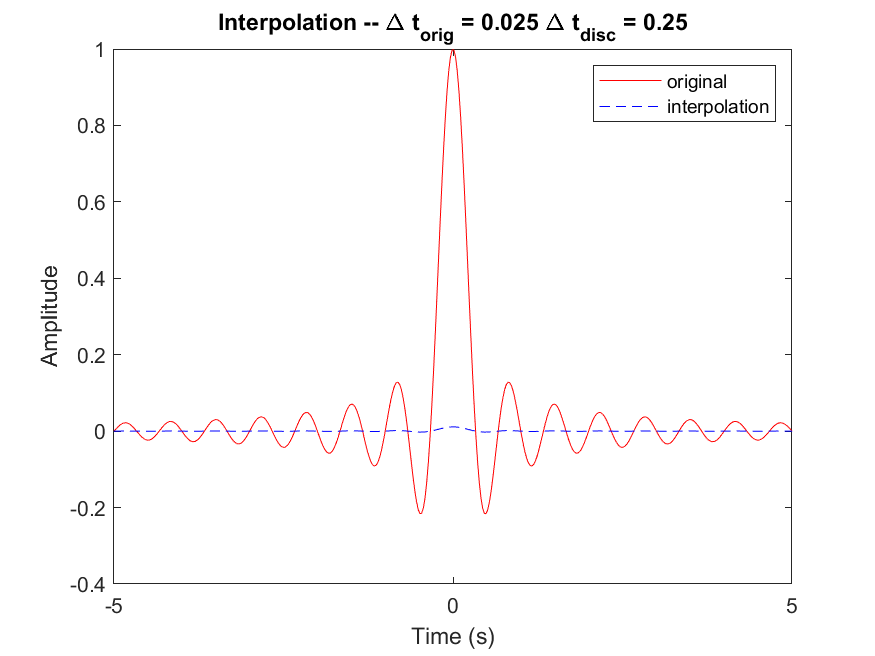
\includegraphics[width=1\textwidth]{2_23.png}
	\end{subfigure}
\hfill
	\begin{subfigure}[b]{0.49\textwidth}
        \centering
		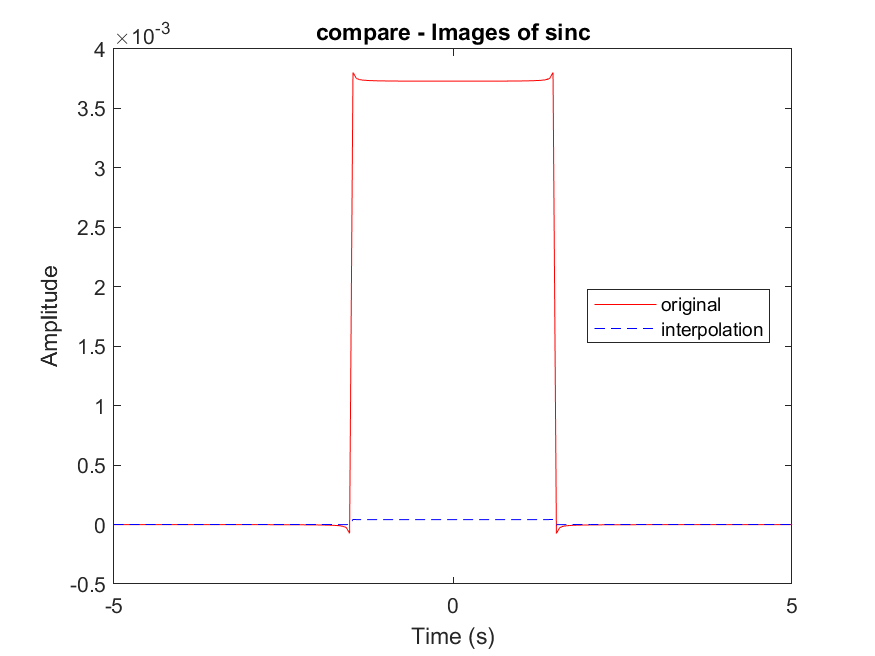
\includegraphics[width=1\textwidth]{2_24.png}
	\end{subfigure}
    \caption{ Испытание - 2 - B = 2}
\end{figure}

\begin{figure}[!ht]
	\centering
\hspace*{\fill}%
	\begin{subfigure}[b]{0.49\textwidth}
        \centering
		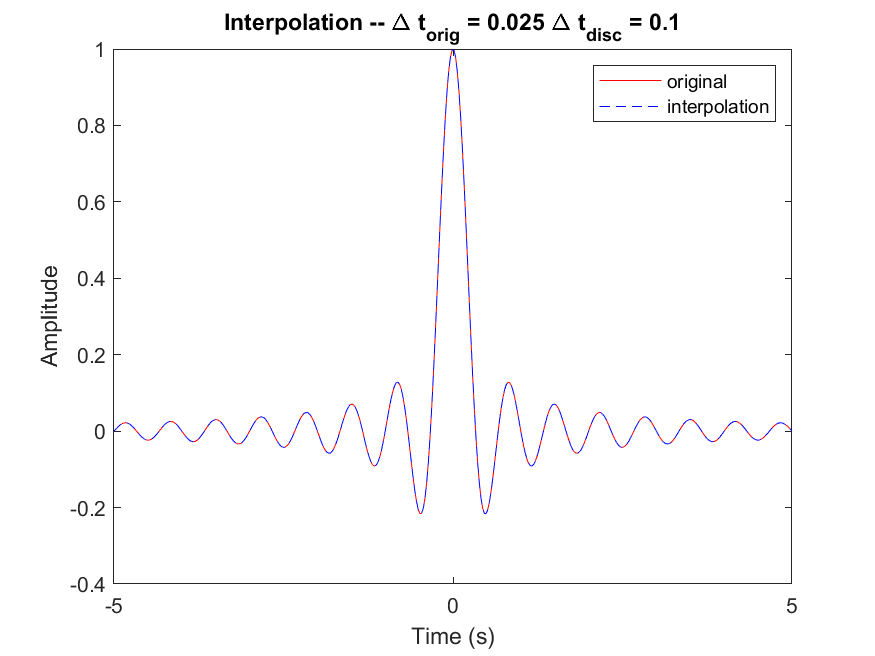
\includegraphics[width=1\textwidth]{2_25.png}
	\end{subfigure}
\hfill
	\begin{subfigure}[b]{0.49\textwidth}
        \centering
		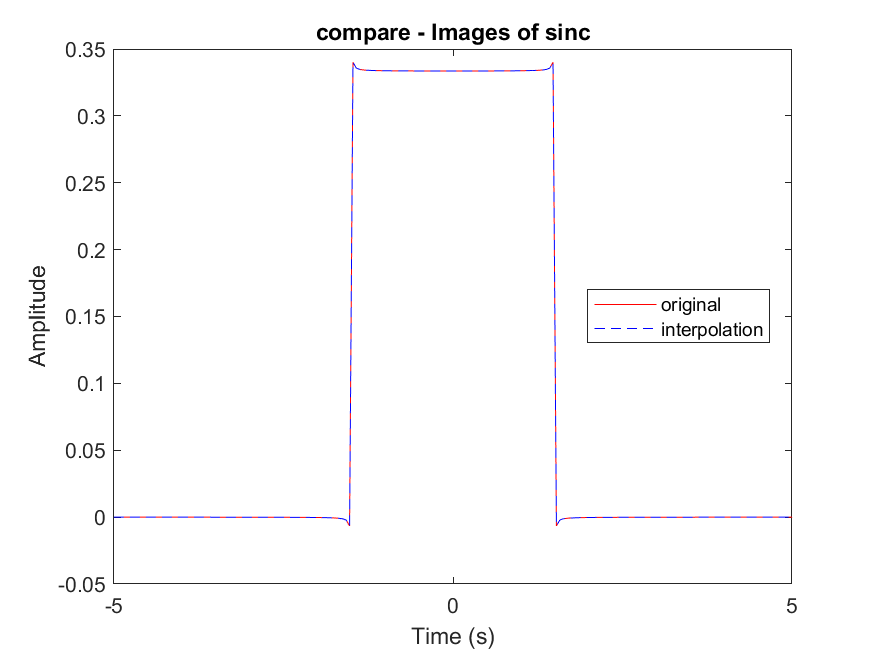
\includegraphics[width=1\textwidth]{2_26.png}
	\end{subfigure}
    \caption{ Испытание - 3 - B = 5}
\end{figure}
\newpage
\begin{figure}[!ht]
	\centering
\hspace*{\fill}%
	\begin{subfigure}[b]{0.49\textwidth}
        \centering
		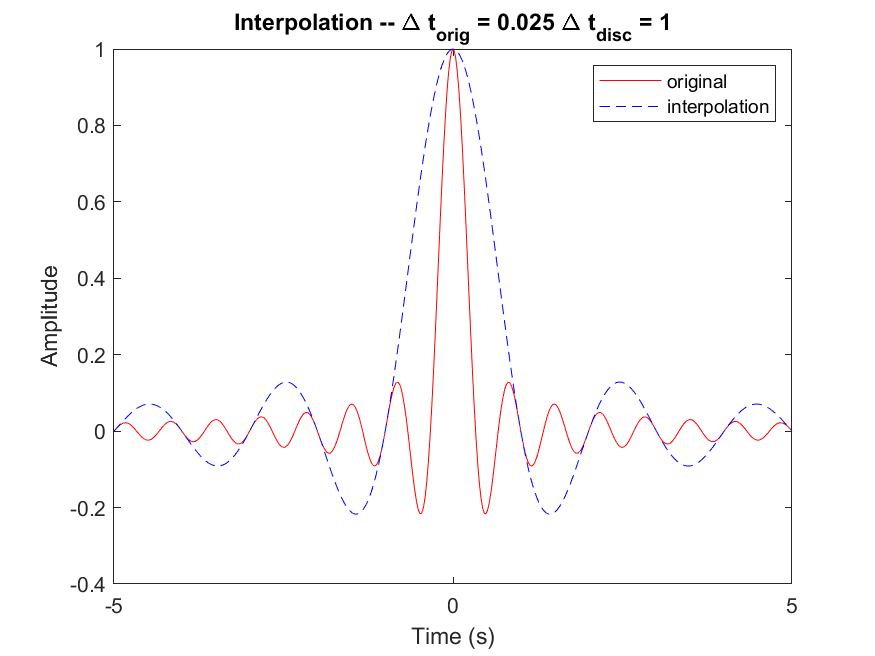
\includegraphics[width=1\textwidth]{2_27.png}
	\end{subfigure}
\hfill
	\begin{subfigure}[b]{0.49\textwidth}
        \centering
		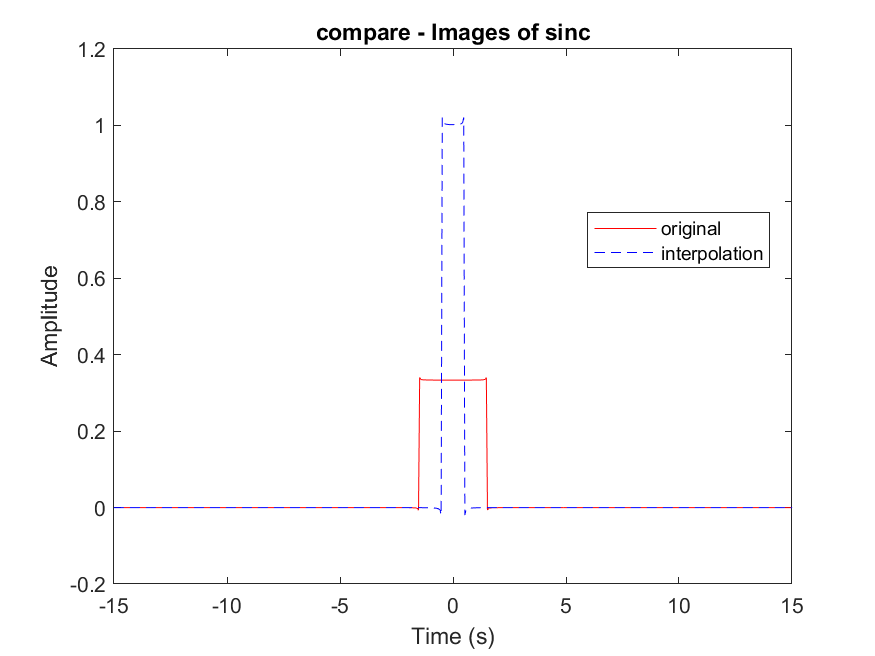
\includegraphics[width=1\textwidth]{2_28.png}
	\end{subfigure}
    \caption{ Испытание - 4 - B = 0.5}
\end{figure}



Мы здесь также проверяли неравенство из теоремы: $\Delta t < \frac{1}{2B}$, где $\Delta t$ -  дискретный шаг времени, 
а $[-B; B]$ - конечный отрезок, в котором лежим весь Фурье образ. В моём случае мы начинали с $B=1$, но я брал и больше и меньше, сравнивая. В случае уже этой функции, она вела себя весьма странно - не всегда уменьшение шага приводило к тому, 
что функция восстанавливалась адекватно, и я, честно, не до конца понимаю как можно такие результаты объяснить

\endinput